\documentclass[12pt]{article}
\usepackage[paper=letterpaper,margin=1.5cm]{geometry}
\usepackage{amsmath}
\usepackage{amssymb}
\usepackage{amsfonts}
\usepackage{mathtools}
\usepackage[utf8]{inputenc}
\usepackage{newtxtext, newtxmath}
\usepackage{enumitem}
\usepackage{titling}
\usepackage{graphicx}
\usepackage[colorlinks=true]{hyperref}
\usepackage{setspace}
\usepackage{braket}
\usepackage{color}
\usepackage{listings}
\usepackage{mathrsfs}
\usepackage{stackengine}

\setstackEOL{\\}

\definecolor{dkgreen}{rgb}{0,0.6,0}
\definecolor{gray}{rgb}{0.5,0.5,0.5}
\definecolor{mauve}{rgb}{0.58,0,0.82}

\lstset{frame=tb,
  language=Python,
  aboveskip=3mm,
  belowskip=3mm,
  showstringspaces=false,
  columns=flexible,
  basicstyle={\small\ttfamily},
  numbers=none,
  numberstyle=\tiny\color{gray},
  keywordstyle=\color{blue},
  commentstyle=\color{dkgreen},
  stringstyle=\color{mauve},
  breaklines=true,
  breakatwhitespace=true,
  tabsize=3
}
\setlength{\droptitle}{-6em}

\newcommand{\hop}{\vspace{1mm}}
\newcommand{\jump}{\vspace{5mm}}
\newcommand{\R}{\mathbb{R}}
\newcommand{\C}{\mathbb{C}}
\newcommand{\bt}{\textbf}
\newcommand{\lm}{\lambda}
\newcommand{\ep}{\varepsilon}
\definecolor{cit}{rgb}{0.05,0.2,0.45}
\addtolength{\jot}{1em}
\newcommand{\solution}[1]{

\vspace{5mm}
\medskip\noindent{\color{cit}\textbf{Solution:} #1}}

\newcounter{tmpctr}
\newcommand\fancyRoman[1]{%
  \setcounter{tmpctr}{#1}%
  \setbox0=\hbox{\kern.1pt\textsf{\Roman{tmpctr}}}%
  \setstackgap{S}{-.2pt}%
  \Shortstack{\rule{\dimexpr\wd0+.1ex}{.5pt}\\\copy0\\
              \rule{\dimexpr\wd0+.1ex}{.5pt}}%
}

\newcommand{\Id}{\fancyRoman{2}}

% Enter the specific assignment number and topic of that assignment below, and replace "Your Name" with your actual name.
\title{STAT 31410: Homework 1}
\author{Caleb Derrickson}
\date{October 8, 2023}

\begin{document}
\onehalfspacing
\maketitle

For this problem set, we consider the equation for an idealized pendulum
\begin{align}
    \frac{d^2\theta}{dt^2} = -\frac{g}{\ell(t)}sin(\theta), \label{Original ode}
\end{align}

where the length of the moment arm, $l$, varies periodically according to

\begin{align}
    \ell (t) = \ell_0(1 + \ep \cos(\omega t)), \hspace{5mm} \ep \ll 1.    \label{length approx}
\end{align}

This might be a good model of a child on a swing, trying to pump energy into it by repeatedly
standing up and then squatting back down with some appropriate rhythm, to be determined.

\jump
\centerline{\noindent}%
\makebox[\textwidth]{
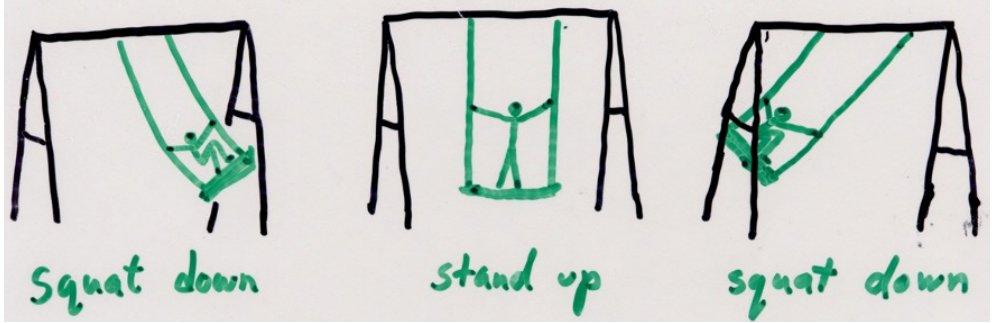
\includegraphics[scale = 0.6]{Images/swing.PNG}
}
\jump

\begin{enumerate}[]
    \item Make an approximation where you keep only the leading order term in $\ep$, i.e linearize about $\varepsilon$ = 0. Then choose a non-dimensionalization of time that puts (1) into this form:

    \begin{align}
        \ddot{\theta} = -(\alpha + \beta \cos(\tau))\sin(\theta),   \label{linearish}
    \end{align}

        where you define the dimensionless parameters $\alpha$ and $\beta$ in terms of the original parameters $g$, $\ell_0$, $\varepsilon$ and $\omega$. Re-write the second order equation \ref{linearish} as two first order equations for the angle $\theta$ and the angular speed $\omega \equiv \dot{\theta}$. For $\beta$ = 0, derive a conserved quantity, the energy of the pendulum, denoted $E(\theta, \Omega)$. Write an equation for $\dot{E}$ that applies if $\beta \neq 0$.

        {\color{cit}\vspace{2mm}\noindent\textbf{Collaborators:}} The TA's of the class, as well as Kevin Hefner, Nathan Suhr, and Steven Lee.
        \begin{solution}

        Since we are taking $\ep \ll 1$ from \ref{Original ode}, we can define a function $f(\ep)$ on which we will expand using ordinary Taylor expansion. Here, I will define $f(\ep)$ as:
        \begin{align}
            f(\ep) = \frac{1}{1 + \ep \cos(\omega t)},
        \end{align}

        where it is understood that $\cos(\omega t)$ is a constant in this sense. Note that we are \textit{linearizing} with respect to $\theta$, so we can drop all terms of higher order. Thus, 

        \begin{align}
            f(\ep) &= \sum_{n = 0}^\infty \ep^n\frac{d^nf}{d\ep^n} \Big\rvert_{\ep = 0} \nonumber \\
            &= f(\ep = 0) + \ep\frac{df}{d\ep} \Big\rvert_{\ep = 0} + O(n^2)  \nonumber \\
            &= 1 - \ep \bigg[ \frac{\cos(\omega t)}{(1 + \ep\cos(\omega t))^2} \bigg]_{\ep = 0}  \nonumber \\
            & = 1 - \ep \cos(\omega t) \label{Expansion} 
        \end{align}

        We can then plug \ref{Expansion} into \ref{Original ode} to obtain,

        \begin{align}
            \ddot{\theta} = -\frac{g}{\ell_0}\Big(1 - \ep \cos(\omega t)\Big)\sin(\theta). \label{before parameters}
        \end{align}

        From \ref{before parameters}, we can define three dimensionless parameters: $\tau, \alpha, \beta$. $\tau$ will take the place of the argument inside the cosine term of \ref{before parameters}, while $\alpha$ and $\beta$ will clean up any extraneous terms. We will first redefine the ratio of $g$ and $\ell_0$ as the resonance frequency of our state, $\omega_0$.
        
        \begin{align*}
            \omega_0^2 = \frac{\ell_0}{g}.    
        \end{align*}

        Then we will take $\tau$ as $\tau = \omega t$. Note that we are taking time derivatives, so this re-parameterization affects what we are differentiating by. 

        \begin{align*}
            \tau = \omega t \implies d\tau = \omega dt \iff \frac{1}{\omega}\frac{d}{d\tau} = \frac{d}{dt}.
        \end{align*}

        Applying these to \ref{before parameters}, we get,

        \begin{align}
            \ddot{\theta} = -\Big(\frac{\omega_0}{\omega} \Big)^2 \big( 1 - \ep \cos(\tau) \big) \sin(\theta).  \label{before alphabeta}
        \end{align}

        We can then define $\alpha, \beta$ as,

        \begin{align}
            \alpha = \bigg(\frac{\omega_0}{\omega}\bigg)^2, \hspace{10mm} \beta = \alpha\ep
        \end{align}

        Note that, as suggested by the TA's, to take $\beta$ as a positive constant. The negative can be recovered by shifting $\tau$ by $\pi$, meaning $\tau = \omega t + \pi$. This shift will change nothing else in our analysis, hopefully. Also, when taking time derivates for the rest of this homework, I am specifically referring to taking the $\tau$ derivative. Thus, our second order differential equation is, 

        \begin{align}
            \ddot{\theta} = -\big(\alpha + \beta \cos(\tau)\big)\sin(\theta),   \label{second order ode with new parameters}
        \end{align}

        matching \ref{linearish}. 

        Our next goal is to re-write \ref{second order ode with new parameters} as two first order equations for $\theta$ and the angular speed $\Omega \equiv \dot{\theta}$. This can be achieved quite easily - our system is now. 
        \begin{equation}
        \begin{cases}
            \dot{\theta} = \Omega, \\
            \dot{\Omega} = -\big(\alpha + \beta \cos(\tau)\big)\sin(\theta) \label{Nonlinear system}
        \end{cases}    
        \end{equation}

        Our next goal is to find a conserved quantity for $\beta = 0$. This quantity will be the energy of our system (or rather, an approximation of it) and will be denoted as $E$. From the lectures, our energy is the sum of kinetic and potential energies, in just the $\theta$ dimension. Potential can be found by integrating the (negative) right-hand-side of \ref{second order ode with new parameters} by our spacial parameter. 

        \begin{align}
            \implies V(\theta) &= \int \alpha\sin(\theta) \ d\theta \nonumber\\
            &= -\big(\alpha + \beta\cos(\tau))\cos(\theta)
        \end{align}

        The energy is now,

        \begin{align}
            E(\theta, \Omega) &= \frac{1}{2} \dot{\theta}^2 + V(\theta),    \nonumber   \\
            E(\theta, \Omega) &= \frac{1}{2} \Omega^2 -\alpha\cos(\theta).
        \end{align}

        Where the instantaneous change in energy (with respect to time) is,

        \begin{align}
            \dot{E}(\theta, \Omega) &=  \frac{d}{d\tau}\bigg[ \frac{1}{2}\Omega^2 - \alpha\cos(\theta) \bigg]  \nonumber\\
            &= \Omega\dot{\Omega} - \alpha\frac{d}{d\tau}\bigg[ \cos(\theta) \bigg] \nonumber\\
            &= -\Omega\big(\alpha + \beta \cos(\tau)\big)\sin(\theta) + \alpha\sin(\theta)\dot{\theta}\nonumber\\
            &= -\beta\Omega\cos(\tau)\sin(\theta) \label{Edot}
        \end{align}
        \end{solution}

        \hrule
        
        \jump
        For the child in the swing picture, is the energy $E$ (instantaneously) increasing or decreasing or neither in each of the frames shown? Try making a rough sketch of the time course of each of these quantities: $\theta(t), \Omega(t), \ell(t)$ and $E(t)$, assuming a periodic motion of the swing as well as the swinger. What is the period of the swing motion compared to the period of $\ell(t)$? Are they the same?

        \begin{solution}
            As a means of faithfully showing the plots, I used matplotlib to create them. Note I am not showing the numerical values of the functions, since they are not enlightening. Note the function $\ell(t)$ is bounded by $1 \pm \ep$. Here is my code:

            \begin{lstlisting}

            import matplotlib.pyplot as plt
            import numpy as np
            import pandas as pd
            %matplotlib inline

            def ell(tau, ep):
                return (1 + ep * np.cos(2 * tau))
            def Omega(tau, ep):
                return -1*(np.sin(tau))
            def energy(tau, ep):
                return 0.5 * Omega(tau, ep) **2 - np.cos(theta(tau))
            def theta(tau):
                return np.cos(tau)

            ep = 0.1
            tau = np.linspace(-np.pi * 2, np.pi * 2, 200)
            tau_ticks = np.arange(-np.pi * 2, np.pi * 2, np.pi/2)
            tau_ticks_label = [f'0' if n == 0 else f'-pi/2' if n == -1 else f'pi/2' if n == 1 else f'{int(n/2)}pi' if n%2 == 0 else f'{int(n)}pi/2' for n in tau_ticks / (np.pi / 2)] 
            
            plt.figure(figsize=(10, 8))
            plt.subplots_adjust(hspace=0.5)
            
            plt.subplot(2, 2, 1)
            plt.plot(tau, ell(tau, ep), 'b-', label = "Length")
            plt.plot(tau, [np.mean(ell(tau, ep)) for _ in range(len(tau))], 'k--')
            plt.xlabel("tau")
            plt.title("Length")
            plt.yticks([])  
            plt.xticks(tau_ticks, tau_ticks_label)
            
            plt.subplot(2, 2, 2)
            plt.plot(tau, Omega(tau, ep), 'r-', label = "Omega")
            plt.plot(tau, 0 * tau, 'k--')
            plt.xlabel("tau")
            plt.title("Omega")
            plt.yticks([])  
            plt.xticks(tau_ticks, tau_ticks_label)
            
            plt.subplot(2, 2, 3)
            plt.plot(tau, energy(tau, ep), 'g-', label = "Energy")
            plt.plot(tau, [np.mean(energy(tau, ep)) for _ in range(len(tau))], 'k--')
            plt.xlabel("tau")
            plt.title("Energy")
            plt.yticks([])  
            plt.xticks(tau_ticks, tau_ticks_label)
            
            plt.subplot(2, 2, 4)
            plt.plot(tau, theta(tau),  'm-', label = "Theta")
            plt.plot(tau, 0 * tau, 'k--')
            plt.xlabel("tau")
            plt.title("Theta")
            plt.yticks([])  
            plt.xticks(tau_ticks, tau_ticks_label)
            
            plt.show()

            \end{lstlisting}

            Here are the resulting plots (I tried making this as horizontally aligned as possible):
            
            \jump
            \centerline{\noindent}%
            \makebox[\textwidth]{
            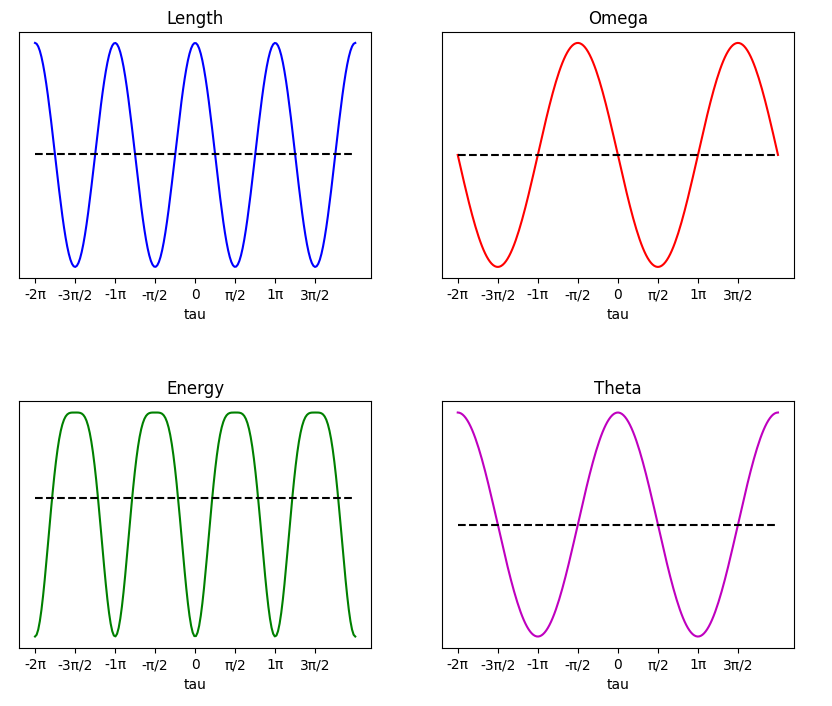
\includegraphics[scale = 0.6]{Images/homework1 heuristic plots.PNG}
            }
            \jump

            Note that these are here purely as a heuristic. As we expect the length of the pendulum arm to be the greatest while the child is squatting down, and minimal when the child to be standing up. Squatting down should correlate to maximum values of theta, and standing up should correlate to minimum values of theta. We can see this represented in the plots of length and theta. Since $\dot{theta} = \Omega$, we should see maxed values of $\omega$ when $\theta$ = 0, which is shown. Energy is slightly different. When $E$ = 0, the kinetic energy is equal to its potential, which happens going to and coming from max values of $\theta$. It's maximal values should then be when either the kinetic or potential energies are maximized, lining up with values $\theta = -\pi/2, 0, \pi/2$. Regardless, in an entire swing interval, when going from $-\pi/2$ to $\pi/2$, we should hit the zeros of $E$ four times, indicating that the energy runs with frequency four times that of $\theta$, twice the frequency of $\ell$. Though this seems to not be represented in the plot of energy, I expect my rationality to be a better interpretation. 

            From our calculation of $\dot{E}$, we can inspect the change of the energy in the given frames of the system. Note that we are to expect the system to achieve its maximum heights in the first and third frames. In the first frame, we can argue the change in energy is zero, as shown by \ref{Edot}, $\Omega$ should be zero. This is also seen in the third frame. The second frame shows the child at $\theta = 0$, thus $\sin(\theta) = 0$, making our $\dot{E}$ also zero. 
        \end{solution}

        \item Linearize your system of first order equations about the equilibrium position $\theta = \Omega = 0$ to obtain a linear non-autonomous system to study:

        \begin{align}
            \frac{d\textbf{x}}{d\tau} = A(\tau)\textbf{x}, \label{Linearized system}
        \end{align}

        where $A(\tau) = A(\tau + T)$ is a 2$\times$2 T-periodic matrix, and $\textbf{x} \in \R^{2}$ is your state space vector. What is T for your non-dimensional problem?
        
        \jump
        \hrule

        \begin{solution}
        
            In preparation for this, we wrote out our ``pseudo system" as \ref{Nonlinear system}. From this, we are only interested in small perturbations of $\theta$ and $\Omega$ around $\theta = \Omega = 0$. Thus, we can replace functions dependent on $\theta$ and $\Omega$ with their Taylor Expanded equivalent, up to linear term. From \ref{Nonlinear system}, the only function is $\sin(\theta)$, which can be approximated by $\sin(\theta) \approx \theta$ under our assumptions. Therefore we have,

            \begin{align}
                \begin{pmatrix}
                    \dot{\theta}    \\
                    \dot{\Omega}
                \end{pmatrix}
                \hspace{3mm}
                =
                \hspace{3mm}
                \begin{pmatrix}
                    0   &1  \\
                    -\big( \alpha + \beta\cos(\tau)\big) &0
                \end{pmatrix}
                \begin{pmatrix}
                    \theta  \\
                    \Omega
                \end{pmatrix}   \label{Linear system}
            \end{align}

            It is quite easy to see that our state vector, \textbf{x} is just $(\theta, \Omega)^t \in \R^2$, where $t$ denotes the transpose. It is also noted that our system $A(\tau)$ is periodic, with period $T = 2\pi$.
        \end{solution}

        \jump
        \hrule
        
        \jump
        Briefly summarize what Floquet theory tells us about the form of the solutions of \ref{Linear system}.

        \begin{solution}
        
            Floquet theory tells us that there exists some periodicity in our solutions. Since our system is periodic (with period $T = 2\pi$), the general form of the solutions is given by theorem 2.36 in the course book.

            \begin{align}
                \upPhi (t,0) = \mathscr{P}(t)e^{tB}, 
            \end{align}

            where $\mathscr{P}$ is a $T$-periodic matrix and $B = \frac{1}{T} \ln M$, where M is the monodromy matrix: $M \equiv \upPhi(T,0)$. 
        \end{solution}

        \item Let $\upPhi(\tau)$ be the fundamental matrix solution associated with the linear problem \ref{Linear system} that satisfies $\upPhi(0) = \Id$, the 2×2 identity matrix. Derive and then solve a first order ordinary differential equation for $det(\upPhi)$.

        \jump
        \hrule

        \begin{solution}
          
        
        \end{solution}
\end{enumerate}
\end{document}
